% !TeX root = ../main.tex

\chapter{研究现状}

\section{深度学习编译概述}

\subsection{深度学习框架}
为了降低深度神经网络的实现难度,研究人员抽象出神经网络的一些通用结构,并由此设计了深度学习框架。下列框架应用较为广泛:

\subsubsection{Caffe \cite{jia2014caffe} }
Caffe (Convolutional Architecture for Fast Feature Embedding) 是 UC Berkeley 使用 C++ 语言开发的开源深度学习框架。代码结构较为简单,易于扩展和调试,主要用于研究和学习。
Facebook 在 2017 年发布了 Caffe2,支持更多的模型。

\subsubsection{TensorFlow \cite{Abadi_TensorFlow_Large-scale_machine_2015}}
TensorFlow 是 Google 开发的端到端开源机器学习平台,有成熟的生态系统和活跃的社区,提供多种编程语言接口,主要用于工业界部署。

\subsubsection{Pytorch \cite{NEURIPS2019_9015} }
Pytorch 是 Facebook 基于 Torch 重写的 Python 深度学习框架,由于其自动求导和反向传播的接口简洁且自然,容易建模,在学术界得到广泛应用。

\subsection{神经网络计算图}
  
在神经网络模型中,同一数据可能被用于多次运算,一次运算也可能需要多条不同的数据。如图 \ref{fig:graph1} 所示,深度学习框架使用计算图(Computational Graph)描述这种多对多关系。

\begin{figure}[h]
    \centering
    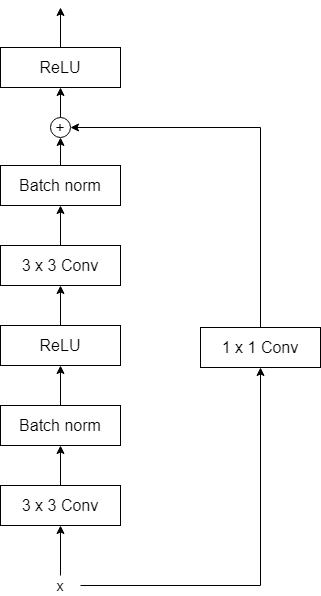
\includegraphics[width=0.4\textwidth]{figures/computational_graph.png}
    \caption{计算图示例}
    \label{fig:graph1}
\end{figure}

计算图有如下性质:

1. 大多数深度学习框架以算子(卷积、全连接等)作为计算图的结点,数据(张量等)作为计算图的边。

2. 计算图可分为静态图和动态图:静态图是指先建立计算图,再输入数据进行计算,这样多次计算使用的是同一张计算图,效率更高;动态图是指计算图随着计算的进行逐渐扩展,灵活性更强。TensorFlow 主要使用静态图,也支持动态图;Pytorch 使用动态图。

3. 计算图是有向无环图。对于有循环结构的神经网络(如 RNN),由于迭代次数有限,也可以将该计算图展开成有向无环图。

4. 从同一结点发出的多条边代表相同的数据被复用多次,因为它们都是该结点的计算结果。

\subsection{深度学习编译器}
\subsubsection{深度学习编译器简介}
深度学习框架的一个重要功能是将高级语言描述的神经网络结构及计算过程转换成不同架构的硬件指令,由于这一过程和传统意义上的编译过程类似,
所以这一部分被称作深度学习编译器\cite{DLcompiler}。以下为常用的深度学习编译器:

\paragraph{XLA \cite{50530}}
XLA (Accelerated Linear Algebra) 是用于加速线性代数运算的领域特定编译器,
它可以在不修改源代码的前提下提高 TensorFlow 和 Pytorch 等框架的模型运行速度,并通过分析和调度程序运行来提高内存利用率。

\paragraph{TVM \cite{DBLP:journals/corr/abs-1802-04799}}
TVM 是一个开源机器学习编译器,用于将不同的高级语言翻译成各种处理器(CPU, GPU, TPU 等)的后端代码,从而实现端到端的代码生成及优化。

\subsubsection{深度学习编译器的中间表示}
同传统的编译器一样,深度学习编译器也需要统一的中间表示(Intermediate Representation, IR)来刻画输入的程序结构。
上文中提到的计算图包含了神经网络的信息,可以作为一种高层次(High-level) IR,但计算图的执行顺序是不唯一的,无法直接被机器使用,需要转化成更低层次(Low-level)的 IR。
以下是一些常见的 IR:
\paragraph{ONNX \cite{onnx}}
ONNX (Open Neural Network Exchange) 是 Facebook 开发的一种机器学习模型的高层表示。该表示与环境和平台无关,可以用于不同深度学习框架的模型保存和载入。
ONNX 使用 Protobuf \cite{enwiki:1061454458} 协议将神经网络的结构和模型参数等信息序列化。
\paragraph{TVM Relay \cite{Relay}}
Relay 是 TVM 团队开发的一种高层 IR,同时支持传统的数据流-控制流描述和函数式编程,相当于一种编程语言,在灵活性上比 ONNX 更强。
\paragraph{MLIR \cite{mlir}}
MLIR (Multi-Level Intermediate Representation) 是 Google 开发的一种编译基础设施,用于生成自定义语言的编译器。使用 MLIR 可以很容易地抽象出不同层次的中间表示,并逐层进行编译优化。

以 XLA 为例,MLIR 使用 Dialect 机制将 XLA 的高层 IR(HLO IR)与 LLVM\cite{enwiki:llvm} (Low Level Virtual Machine,一种编译器基础设施) IR 统一到一个框架中,降低了构建专用编译器的成本。

\subsection{深度学习编译器的优化策略}
计算图构建完成后,编译器前端会对计算图进行图级别的优化。图级别的优化主要考虑结点的特征和图的拓扑结构,
编译器后端则会针对目标硬件的特点,进行体系结构相关的优化。后端优化策略主要有两种:一种是将低层 IR 转换成 LLVM IR,从而利用 LLVM 生成汇编代码,另一种策略是根据深度学习的领域特定知识和目标硬件的特点,定制更高效的编译器后端。

以下为一些优化策略的例子 \cite{DLcompiler}:

\subsubsection{编译器前端进行的优化}
\paragraph{Node elimination}
无用结点消除是指根据输入数据的实际情况,消除没有实际意义的计算结点,如只有一个输入元素的 sum 结点。
\paragraph{Operator fusion}
算子融合是指将多个原子操作对应的算子合并成一个算子,从而可以有效利用计算的中间结果,降低数据传输带来的开销。
为找到能够融合的算子,编译器需要识别复杂的子图模式,也需要权衡如何划分算子组合才能得到最优的性能。

\subsubsection{编译器后端进行的优化}
\paragraph{Memory latency hiding}
访存延时隐藏是指设计运算的并行顺序,使得在准备某些运算所需数据的访存过程中,可以进行其他不相关的运算,从而减少了运算总时间。
\paragraph{Tiling}
瓦片化是指由于目标硬件的缓存大小有限,编译器将大循环分割成一些小循环,从而更好地利用程序的局部性。因为不同目标硬件的缓存大小不同,
编译器需要对小循环的大小进行不同的尝试。

\newpage
\section{计算图耗时预测模型}

\subsection{传统模型}

传统耗时预测方法 Paleo \cite{Paleo} 使用如下经验公式预测计算图单个结点 $v$ 的执行时间:
\begin{align}
  T(v) = \sum \limits_{(u, v) \in \mathcal{E}}
  \mathcal{R} (u) + \mathcal{C}(f_v,d_v) + \mathcal{W}(f_v,d_v)
\end{align}
其中 $\mathcal{R}(u)$ 表示 $v$ 从前驱结点 $u$ 获取数据所需的时间。
$\mathcal{C}(f_v,d_v)$ 表示 $v$ 对应算子 $f_v$ 在给定硬件 $d_v$ 上计算所需时间,
可以用 $f_v$ 所需进行的浮点运算次数与 $d_v$ 的运算速度的比值估计。
$\mathcal{W}(f_v,d_v)$ 表示把运算结果写入 $d_v$ 的存储器所需要的时间。

对于整个计算图,耗时模型为其添加整体的源节点和汇结点,从而将运算图分为并行和串行的部分。
耗时模型会将并行的部分合并为一个结点,该结点的执行时间在各个并行部分执行时间的最大值和总和之间(由设备并行度决定)。
最后耗时模型将所有串行的部分所需时间相加得到整个计算图的运行时间。

Paleo 的处理流程如图 \ref{fig:graph2} 所示:
\begin{figure}[h]
  \centering
  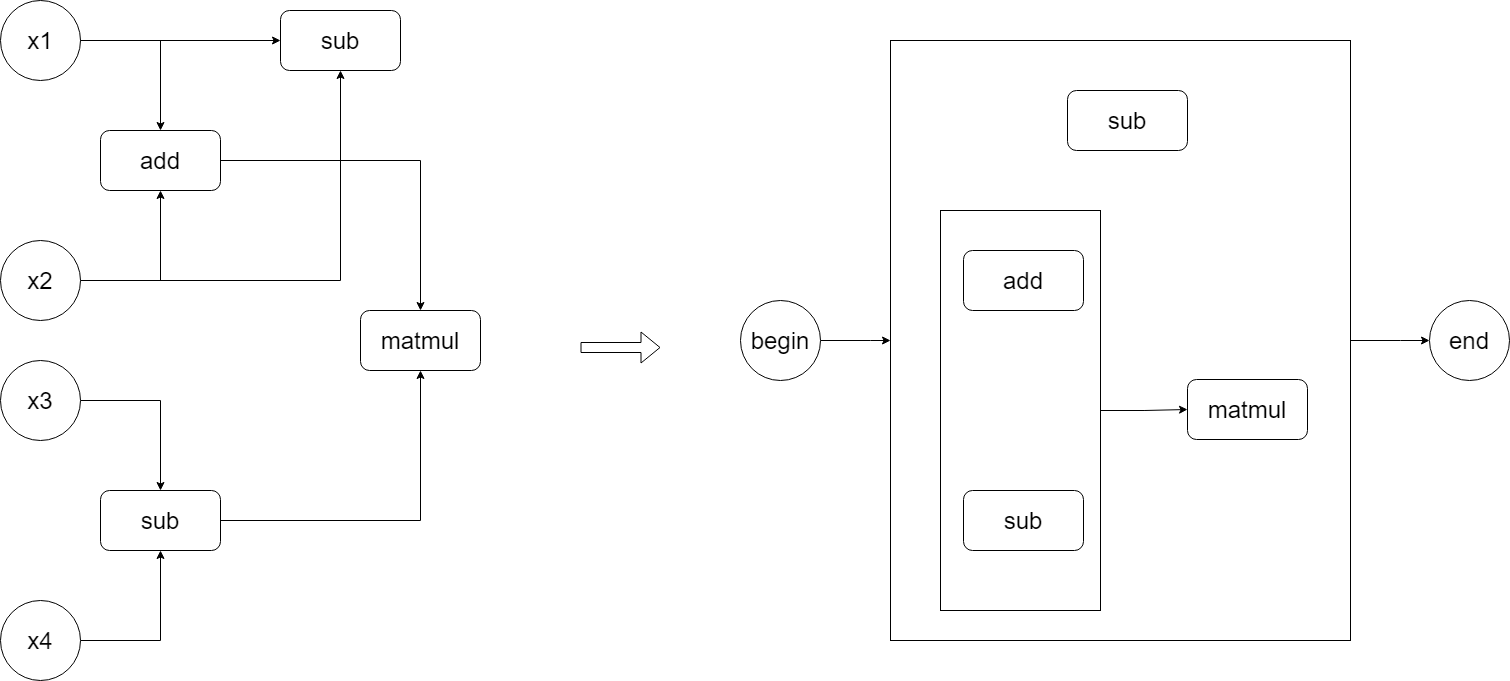
\includegraphics[width=1\textwidth]{figures/graph2.png}
  \caption{Paleo 的处理流程}
  \label{fig:graph2}
\end{figure}

\subsection{LSTM 模型}

长短期记忆\cite{LSTM_origin}(Long short-term memory, LSTM)模型是一种能够处理长期时间序列输入的循环神经网络\cite{RNN}(Recurrent neural network, RNN)。

假设单核处理器按照任意拓扑排序执行计算图的每个结点,则这些结点可以看作时间序列,故 Facebook 等团队 \cite{LSTM1} \cite{LSTM2} 提出使用长短期记忆模型估计计算图的运行时间。
但对于可以并行执行多个结点的多核处理器,这种方法相当于为并行执行的多个结点添加了额外的顺序信息,会影响预测的准确性。

一种解决方案 \cite{LSTM1} 是使用 DAG-RNN \cite{DAG-RNN} 模型:仍按照任意拓扑序处理计算图的每个结点,但当遇到某个结点有多个前驱时,对它所有前驱的隐层向量按分量取最大值,作为该结点的隐层向量。
原因是如果多个结点可以并行执行,则总时间取决于执行时间最长的结点。最后将所有出度为 0 的结点的隐层向量按分量取最大值,作为整个计算图的特征向量,再将其通过一个全连接层得到运行时间预测结果。

DAG-RNN 的处理流程如图 \ref{fig:graph3} 所示:

\begin{figure}[h]
    \centering
    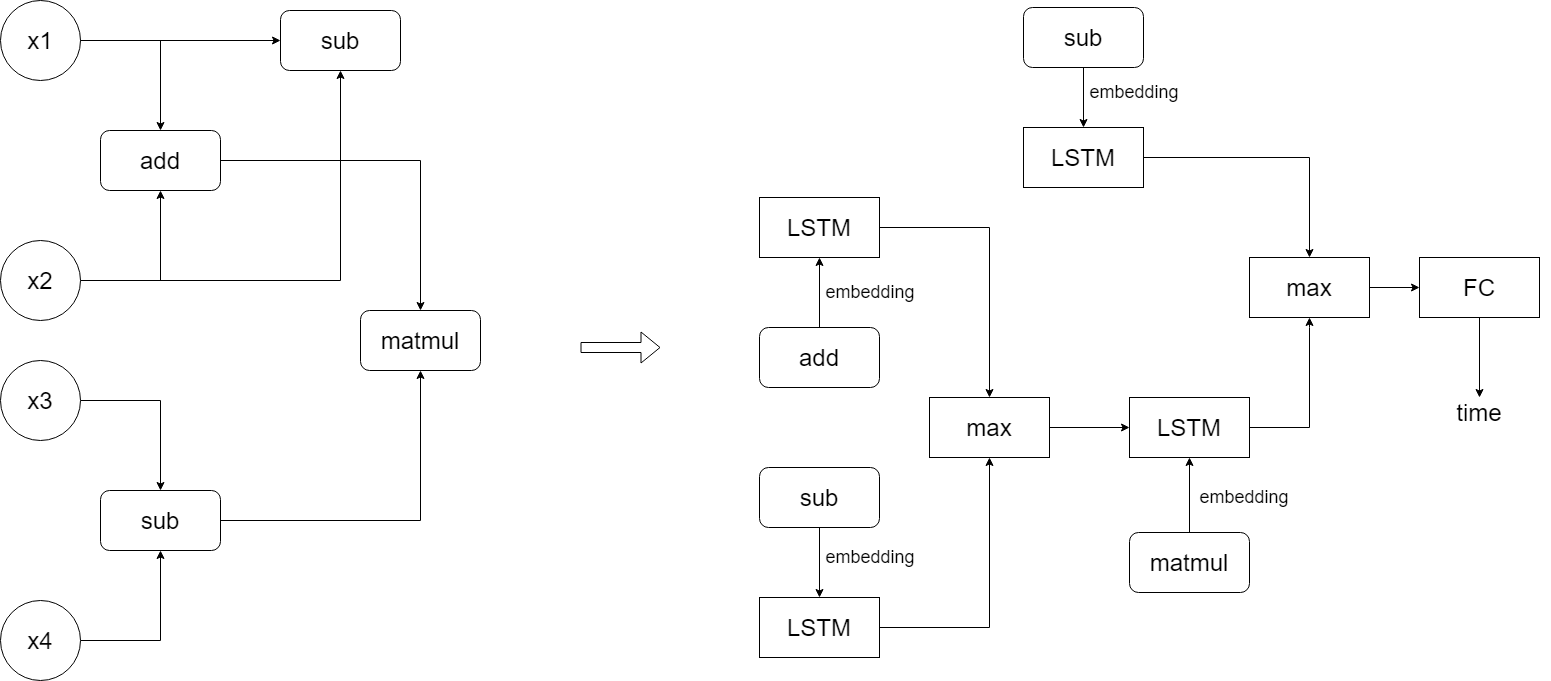
\includegraphics[width=1\textwidth]{figures/graph1.png}
    \caption{DAG-RNN 的处理流程}
    \label{fig:graph3}
\end{figure}

\subsection{图神经网络模型}

图神经网络(Graph Neural Networks,GNN)\cite{GNN}是一类处理图数据的神经网络结构。图神经网络的一个重要应用是生成结点嵌入(node embeddings),
即用每个结点邻居的嵌入向量来影响该结点的嵌入向量,从而充分利用图的拓扑结构,使得每个结点学习出更准确的向量表示。

以下是一些常见的图神经网络模型:

\begin{figure}
    \centering
    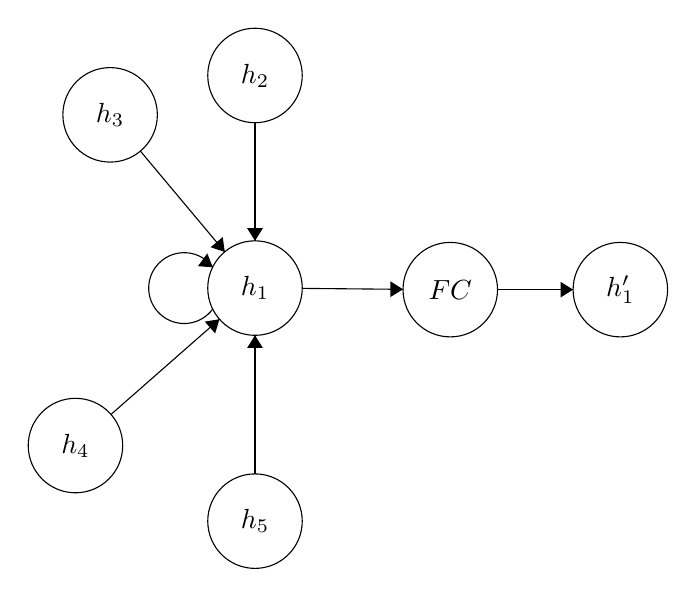
\begin{tikzpicture}[scale=0.2]
    \tikzstyle{every node}+=[inner sep=0pt]
    \draw [black] (24.4,-30.6) circle (3);
    \draw (24.4,-30.6) node {$h_1$};
    \draw [black] (24.4,-17.1) circle (3);
    \draw (24.4,-17.1) node {$h_2$};
    \draw [black] (15.2,-19.6) circle (3);
    \draw (15.2,-19.6) node {$h_3$};
    \draw [black] (13,-40.6) circle (3);
    \draw (13,-40.6) node {$h_4$};
    \draw [black] (24.4,-45.4) circle (3);
    \draw (24.4,-45.4) node {$h_5$};
    \draw [black] (36.8,-30.7) circle (3);
    \draw (36.8,-30.7) node {$FC$};
    \draw [black] (47.6,-30.7) circle (3);
    \draw (47.6,-30.7) node {$h_1'$};
    \draw [black] (24.4,-20.1) -- (24.4,-27.6);
    \fill [black] (24.4,-27.6) -- (24.9,-26.8) -- (23.9,-26.8);
    \draw [black] (17.12,-21.9) -- (22.48,-28.3);
    \fill [black] (22.48,-28.3) -- (22.35,-27.36) -- (21.58,-28.01);
    \draw [black] (15.26,-38.62) -- (22.14,-32.58);
    \fill [black] (22.14,-32.58) -- (21.21,-32.73) -- (21.87,-33.48);
    \draw [black] (24.4,-42.4) -- (24.4,-33.6);
    \fill [black] (24.4,-33.6) -- (23.9,-34.4) -- (24.9,-34.4);
    \draw [black] (21.72,-31.923) arc (-36:-324:2.25);
    \fill [black] (21.72,-29.28) -- (21.37,-28.4) -- (20.78,-29.21);
    \draw [black] (27.4,-30.62) -- (33.8,-30.68);
    \fill [black] (33.8,-30.68) -- (33,-30.17) -- (33,-31.17);
    \draw [black] (39.8,-30.7) -- (44.6,-30.7);
    \fill [black] (44.6,-30.7) -- (43.8,-30.2) -- (43.8,-31.2);
    \end{tikzpicture}
    \caption{图神经网络示意图} 
    \label{fig:graph4}
\end{figure}

\subsubsection{GCN}
卷积图神经网络\cite{GCN}(Graph Convolutional Network, GCN)是一种将传统的卷积神经网络\cite{CNN}(Convolutional neural network, CNN)应用到图空间的方法。
传统的卷积操作的作用是带权采样欧几里得空间中某个元素及其邻域内的特征,并将这些元素合并成一个以上述采样为特征的新元素。

对于图空间,一次卷积操作使用某个结点与其相邻结点的嵌入向量的平均值作为其聚合结果,该结果经过一个全连接层用于提取特征和降低嵌入向量的维度,得到卷积操作的输出:
\begin{equation}
    H^{(l+1)} = \sigma(\tilde{D}^{-\frac 12}\tilde{A}\tilde{D}^{-\frac 12}H^{(l)}W^{(l)}).
\end{equation}
其中,$\tilde{A} = A + I$ 为添加自环的邻接矩阵。$\tilde{D} = \sum_{j} \tilde{A_{ij}}$ 用于对 $\tilde{A}$ 归一化,从而实现对邻域求平均的操作。$H^{(l)}$ 为第 $l$ 层所有结点的嵌入向量。$W^{(l)}$ 为第 $l$ 层的全连接矩阵,是可以学习的参数。$\sigma$ 为激活函数。

海康威视\cite{haikang},Facebook\cite{GCN2} 等团队采用卷积图神经网络的方法获取结点的嵌入向量,进而对神经网络的运行时间进行估计。

\subsubsection{GraphSAGE}

GraphSAGE \cite{GraphSAGE} 是一种基于归纳推理的结点嵌入方法。与 GCN 相比,GraphSAGE 更适合处理不断延伸出新结点的图,原因是 GraphSAGE 不使用邻接矩阵进行统一计算,而是分别对每个结点进行聚合操作,这样在出现新节点时就无需重新计算所有结点嵌入。

此外,GraphSAGE 不使用结点的所有邻居信息,而是进行随机采样,从而提高了效率。
如果 GraphSAGE 的聚合函数是平均值函数,则效果和 GCN 类似,但 GraphSAGE 的聚合函数还可以是 LSTM 或 Pooling 等可导算子。

以下为 GraphSAGE 的伪代码 \cite{GraphSAGE}。

\begin{algorithm}[H]
    \caption{GraphSAGE}
    \label{alg:GraphSAGE}
    \SetKwInOut{Input}{Input}\SetKwInOut{Output}{Output}
    \Input{图 $\mathcal G(\mathcal V,\mathcal E)$;输入特征 $\{\mathbf{x}_v, \forall v\in \mathcal V\}$; 深度 $K$; 权重矩阵 $\mathbf{W}^{k}, \forall k \in \{1,...,K\}$; 激活函数 $\sigma$; 聚合函数 $\textsc{AGGREGATE}_k, \forall k \in \{1,...,K\}$; 邻居集合 $\mathcal{N} : v \rightarrow 2^{\mathcal V}$}
    \Output{嵌入向量 $\mathbf{z}_v$ for all $v \in \mathcal V$}
    \BlankLine
    $\mathbf{h}^0_v \leftarrow \mathbf{x}_v, \forall v \in \mathcal V$ \;
    \For{$k=1...K$}{
          \For{$v \in \mathcal V$}{
          $\mathbf{h}^{k}_{\mathcal{N}(v)} \leftarrow \textsc{AGGREGATE}_k(\{\mathbf{h}_u^{k-1}, \forall u \in \mathcal{N}(v)\})$\;
                  $\mathbf{h}^k_v \leftarrow \sigma\left(\mathbf{W}^{k}\cdot \textsc{CONCAT}(\mathbf{h}_v^{k-1}, \mathbf{h}^{k}_{\mathcal{N}(v)})\right)$
          }
          $\mathbf{h}^{k}_v\leftarrow \mathbf{h}^{k}_v/ \|\mathbf{h}^{k}_v\|_2, \forall v \in \mathcal V$
        }
     $\mathbf{z}_v\leftarrow \mathbf{h}^{K}_v, \forall v \in \mathcal{V}$ 
\end{algorithm}
谷歌 \cite{Alearned} 团队采用 GraphSAGE 的方法对神经网络的运行时间进行估计。

\subsubsection{利用边特征的图神经网络}
上述图神经网络模型只利用了图的结点特征,为了处理计算图边上的张量特征,本文尝试的能够同时聚合边上和结点特征的图神经网络结构\cite{EdgeGNN} 如下:

\paragraph{使用多层感知机聚合结点和边的特征\cite{MLPEdgeGNN}}

一个自然的想法是在算法 \ref{alg:GraphSAGE} 的聚合函数之前添加一个可学习的函数,
从而将每条边的嵌入向量聚合到它的头节点中,即
\begin{equation}
    h_{u}^{k-1} \leftarrow \phi(h_u^{k-1}, h_{(u,v)}^{k-1})
\end{equation}
由于多层感知机\cite{MLP}可以很好地拟合任意函数,故本文将边的嵌入向量与其头节点的嵌入向量拼接后通过一个多层感知机,得到该头节点用于聚合的嵌入向量。

\paragraph{CFConv \cite{SchNet}}

CFConv 是 SchNet \cite{SchNet} 中使用的一种用于聚集结点和边上特征的图神经网络结构。与多层感知机类似,CFConv 使用一个可学习的变换矩阵将边的嵌入向量映射成和结点的嵌入向量等维度的向量,
再与结点的嵌入向量做逐元素乘法,最后进行聚合。其计算过程如下:
\begin{equation}
    h_u^{k} = \mathbf{SSP}(\sum \limits_{v \in \mathcal{N}(u)} h_v^{k-1} \circ W^{k-1} h^{k-1}_{(u,v)})
\end{equation}
其中,$\circ$ 表示向量逐元素乘法,SSP 为激活函数,其计算公式如下:
\begin{align}
    \mathbf{SSP}(x) = \frac{1}{\beta} * \log(1 + \exp(\beta * x)) - \log(\mathbf{shift})
\end{align}
